%
% File acl2021.tex
%
%% Based on the style files for EMNLP 2020, which were
%% Based on the style files for ACL 2020, which were
%% Based on the style files for ACL 2018, NAACL 2018/19, which were
%% Based on the style files for ACL-2015, with some improvements
%%  taken from the NAACL-2016 style
%% Based on the style files for ACL-2014, which were, in turn,
%% based on ACL-2013, ACL-2012, ACL-2011, ACL-2010, ACL-IJCNLP-2009,
%% EACL-2009, IJCNLP-2008...
%% Based on the style files for EACL 2006 by 
%%e.agirre@ehu.es or Sergi.Balari@uab.es
%% and that of ACL 08 by Joakim Nivre and Noah Smith

\documentclass[11pt,a4paper]{article}
\usepackage[hyperref]{acl2021}
\usepackage{times}
\usepackage{latexsym}
\usepackage{booktabs}
\usepackage{multirow}
\usepackage{graphicx}
\usepackage{amsmath}
\usepackage{amsfonts}
\graphicspath{{figures/}}
\usepackage{algorithm}
\usepackage{algpseudocode}
\usepackage{float}
\usepackage{stfloats}
\usepackage{alltt}
\usepackage{verbatim}
\usepackage{graphicx}
\usepackage{wrapfig}
\usepackage{subcaption}
\usepackage[table]{xcolor}
\usepackage{makecell}

\renewcommand{\UrlFont}{\ttfamily\small}

\usepackage{microtype}
\usepackage{xcolor}

\usepackage{listings}
\lstset{basicstyle=\ttfamily, columns=flexible, breaklines=true, mathescape=true}
\usepackage{courier}
\usepackage{float}

\newcommand{\TODO}[1]{\textcolor{red}{TODO: #1}}

\aclfinalcopy % Uncomment this line for the final submission

\newcommand\BibTeX{B\textsc{ib}\TeX}

% Formal notation
\renewcommand{\S}{\mathcal{S}}
\newcommand{\R}{\mathcal{R}}
\newcommand{\T}{\mathcal{T}}
\newcommand{\A}{\mathcal{A}}
\renewcommand{\P}{\mathcal{P}}

\usepackage[english]{babel}
\renewcommand{\sectionautorefname}{Section}
\renewcommand{\subsectionautorefname}{Section}
\renewcommand{\subsubsectionautorefname}{Section}

% Box for ai generated text
\usepackage[most]{tcolorbox}
\newtcblisting{aibox}[2][]{%
  colback=gray!2!white,
  colframe=black,
  title={#2}, 
  #1
}
\newcommand{\red}[1]{\colorbox{red!25!white}{#1}}

\title{Predicting spread of Alzheimer’s disease pathology using brain  connectomes from different cognitive stages}
\author{Melina Jingting binti Laimon}
\date{\today}

\begin{document}
\maketitle
\begin{abstract}
    
\end{abstract}

\section{Introduction}
\label{sec:Introduction}

Alzheimer’s disease (AD) is a progressive neurodegenerative disorder and the leading cause of dementia worldwide, affecting tens of millions of people and placing an enormous burden on public health \citep{yuHumanConnectomeAlzheimer2021}. Pathologically, AD is characterized by the accumulation of amyloid-$\beta$ (A$\beta$) plaques and tau protein neurofibrillary tangles, which disrupt synaptic function and ultimately drive extensive neuronal loss \citep{goedertAlzheimersParkinsonsDiseases2015, weickenmeierPhysicsbasedModelExplains2019}. Despite concerted research efforts, effective disease-modifying treatments remain elusive, in part owing to the complexity and heterogeneity of AD progression \citep{yuHumanConnectomeAlzheimer2021}. Enhanced mechanistic understanding of how tau pathology spreads, and how A$\beta$ may trigger or accelerate this spread, is therefore crucial for developing earlier diagnostic strategies and more effective interventions. \\

 Tau-propagation models are often based on the \textbf{prion hypothesis}, based on evidence indicates that misfolded proteins such as tau propagate trans-synaptically in a prion-like fashion from vulnerable epicenters to connected brain regions, giving rise to the characteristic Braak staging patterns documented in pathological and PET imaging studies \citep{vogelConnectomebasedModellingNeurodegenerative2023, rajNetworkDiffusionModel2012}. Researchers have thus increasingly turned to \emph{network-based} computational models—relying on connectomics—to better understand how tau spreads via large-scale anatomical or functional pathways in the brain \citep{rajNetworkDiffusionModel2012,toxtobyDataDrivenSequenceChanges2017,weickenmeierPhysicsbasedModelExplains2019,heCoupledmechanismsModellingFramework2023, hompsonCombiningMultimodalConnectivity2024}.\\

 \textbf{The amyloid cascade hypothesis} posits that pathological aggregation of A$\beta$ initiates a cascade culminating in tau-mediated neurodegeneration \citep{goedertAlzheimersParkinsonsDiseases2015}. Indeed, early A$\beta$ deposition correlates with downstream metabolic and cellular changes that promote tau seeding and aggregation. This synergy helps to explain why tau pathology emerges in close spatiotemporal association with cortical amyloid burden \citep{bielCombiningTauPETFMRI2022}.\\

\textbf{Predictive accuracy of models across cognitive stages is unclear.} a pivotal question in these modeling efforts is whether to employ template (group-averaged) connectomes or patient-specific connectomes \citep{thompsonPredictingSpreadAlzheimers, vasaNullModelsNetwork2022}. Although group-level templates can simplify modeling and reduce noise, each individual’s connectome exhibits unique topological features that might shape disease spread. Meanwhile, most existing approaches apply a single model across heterogeneous cohorts or focus only on one disease stage. Consequently, it remains unclear whether predictive accuracy differ between early asymptomatic or mild cognitive impairment (MCI) stages versus frank AD dementia \citep{heCoupledmechanismsModellingFramework2023}. Moreover, standard network diffusion models often ignore local factors, such as amyloid load, that can modulate tau progression.\\

To address these gaps, we systematically compare three models for predicting tau spread across the Alzheimer’s disease spectrum. Specifically, we evaluate the performance of Network Diffusion Model (NDM), Fisher--Kolmogorov--Petrovsky--Piscounov (FKPP), and a weighted FKPP model that incorporates regional A$\beta$ burden in connectomes derived from participants across four cognitive stages: cognitively normal (CN), early MCI (EMCI), late MCI (LMCI), and probable AD (AD). By examining how each model performs at each disease stage, we aim to provide insights into the mechanisms and predictive power of network-based disease spread models, as well as clarify the role of amyloid-tau interactions in shaping the topography of tau deposition \citep{thompsonDemonstrationOpensourceToolbox2024}. In doing so, we seek a more comprehensive perspective on AD progression across the clinical continuum and a foundation for future personalized modeling efforts.





\section{Methods}
\label{sec:Methods}

\subsection{Data}

\subsubsection{Connectomes}
We used structural connectomes for 168 participants in the Alzheimer’s Disease Neuroimaging Initiative (ADNI)\footnote{\url{https://adni.loni.usc.edu}} database, evenly distributed across four cognitive stages: cognitively normal (CN), early mild cognitive impairment (EMCI), late mild cognitive impairment (LMCI), and probable Alzheimer’s disease (AD). Each group thus contained 42 participants. For each individual, diffusion MRI and tractography were used to reconstruct whole-brain white matter fibers and generate a weighted, undirected connectivity matrix \citep{oxtobyDataDrivenSequenceChanges2017}. These matrices have node labels corresponding to cortical (and some subcortical) regions of interest, following a predefined parcellation scheme, and edge weights representing the number of streamlines between each pair of regions.

\subsubsection{Tau PET data}\label{section:tau_data}
We used tau PET scans from 242 ADNI participants who were classified as having elevated tau levels. We used group-averaged tau PET signals by averaging SUVR values across 242 individuals. These aggregated tau maps served as the “ground truth” against which we fit our various disease-spread models.

\subsubsection{Amyloid PET data}\label{section:amyloid_data}
We also incorporated group-averaged amyloid-beta (A$\beta$) measures (SUVRs) from 241 participants. Amyloid burden is widely believed to initiate upstream in the pathological cascade, potentially catalyzing or accelerating tau aggregation \citep{heCoupledmechanismsModellingFramework2023, weickenmeierPhysicsbasedModelExplains2019}. We therefore leveraged these A$\beta$ SUVR values to weight the local production term in our A$\beta$-FKPP model (see Section~\ref{sec:WeightedFKPP}). For subcortical regions, the amyloid PET intensities have been set to 1 (i.e., no additional weighting) to account for inaccuracies in measuring A$\beta$ in deep structures.

\subsection{Connectome Metrics using the Brain Connectivity Toolbox}\label{section:connectome_metrics}
For each individual's structural connectome, we computed all metrics listed below using the Python implementation of the Brain Connectivity Toolbox (BCT). \\

Before calculating the metrics, each connectome matrix was min-max normalized. This normalization was applied to ensure that differences in overall connection strength between individuals did not bias the graph metrics, allowing for more valid comparisons across participants and groups. We verified that all metrics were computed using weighted undirected versions of the functions in BCT.\\

For node-level metrics, specifically, node strength and clustering coefficient, we compared the mean values across all nodes as well as conducted between-node analyses. With a large number of 84 nodes, we focus the comparisons made by first conducting Kruskal–Wallis tests across all nodes, and then performing Dunn’s post-hoc tests only on the single node with the lowest KW p-value. Statistical tests are elaborated in Section~\ref{section:statistical_tests}.\\

\subsubsection{Metrics}\label{section:connectome_metrics}
\begin{itemize}
    \item \textbf{Node strength}: The sum of the weights of all edges connected to a node. This indicates how strongly connected or “well-networked” a region is within the connectome. Nodes with high strength serve as hubs. In the context of pathology, such hubs could accumulate tau from multiple inputs or facilitate its wide dissemination to other regions due to their numerous strong connections.
    \item \textbf{Clustering coefficient}: The fraction of a node’s neighbors that are also interconnected with each other. This measures the prevalence of tightly knit clusters (triangles) in the network around that node. This local interconnectedness might influence tau propagation by creating short loops for re-circulating or amplifying tau in a region’s vicinity.
    \item \textbf{Global efficiency}: The average of the inverse shortest path lengths between all pairs of nodes. This reflects how efficiently information (or in this case, a spreading agent like tau) can be transferred across the whole brain network.
    \item \textbf{Diffusion efficiency}: The inverse of the mean first-passage time for a random walker to travel between nodes on the network. This quantifies how quickly, on average, a signal (or tau protein) can reach any region from any other region via the connectome.
    \item \textbf{Density}: The ratio of existing edges to possible edges in the network, ignoring weights. A higher density implies more pathways along which tau pathology can travel.
\end{itemize}

\subsubsection{Statistical test}\label{section:statistical_tests}
We used the Kruskal-Wallis test as implemented in Scipy\footnote{\url{https://scipy.org/}} to assess whether the distributions of each connectome metric differed significantly across the four cognitive groups. This non-parametric test is appropriate given the non-normality of our data. We then performed Dunn's post-hoc tests as implemented in Scikit-learn\footnote{\url{https://scikit-learn.org/}} to identify which specific groups differed from each other, applying a Bonferroni correction for multiple comparisons.

\subsection{Tau Propagation Models using the Network Spreading Models Toolbox}
We modelled connectivity-mediated tau propagation using the Network Spreading Models (NSM) Toolbox \citep{thompsonDemonstrationOpensourceToolbox2024}, using specifically the toolbox's implementation of the models NDM, FKPP, weighted FKPP and model selection metric AICc.

\subsubsection{Models}
\begin{itemize}
    \item \textbf{NDM}:
    We use the network diffusion model (NDM) as the baseline. NDM as proposed in \citet{rajNetworkDiffusionModel2012} models the prion-like diffusion of tau based on connectivity. The model is defined as:
    $$
        \frac{d\mathbf{x}(t)}{dt} = -\beta H \mathbf{x}(t)
    $$
    where $\mathbf{x}(t)$ is the regional pathology at time $t$, $\beta$ is the diffusion constant, and $H$ connectome Laplacian. We set the diffusion constant $\beta$ to 1, since we are not calibrating the model to any specific time scale.

    \item \textbf{FKPP}:
    The Fisher-Kolmogoroc-Petrovsky-Piscounov FKPP \citep{weickenmeierPhysicsbasedModelExplains2019} couples diffusive propagation of tau with local logistic growth, and is expressed as:
    $$
    \frac{d\mathbf{x}(t)}{dt}
    =
    -\alpha H \mathbf{x}(t)
    +
    (1-\alpha)\mathbf{x}(t)(1-\mathbf{x}(t))
    $$
    Where $\alpha$ is the weight for spread contribution.

    \item \textbf{Weighted-FKPP}\label{section:WeightedFKPP}: 
    The Weighted-FKPP extends the basic FKPP equation by allowing for differing tau production levels at each node \citep{heCoupledmechanismsModellingFramework2023}. In our case, we scale the local growth term according to the local amyloid-$\beta$ (A$\beta$) level. For the rest of this paper, we will refer to this model as the \textbf{A$\beta$-FKPP}.
    $$
    \frac{d\mathbf{x}(t)}{dt}
    =
    -\alpha H \mathbf{x}(t)
    +
    \mathbf{v}(1-\alpha)\mathbf{x}(t)(1-\mathbf{x}(t))
    $$
    where $\mathbf{v}$ is a vector of regional production weights, and is set to be the local A$\beta$ level.
\end{itemize}


\subsubsection{Hyperparameter optimization}
There are two key hyperparameters for these models: the seed region and the timepoint. The set of candidate seed regions is constrained to be hemisphere-agnostic, thereby reducing the number of nodes from 84 to 42. The candidate timepoints are defined within the range 0 to 50 in increments of 0.1, over which the model's performance is evaluated.\\ 

In the Network Diffusion Model (NDM), the NSM Toolbox identifies the optimal seed region and timepoint via a grid search. In contrast, for the FKPP and Weighted-FKPP models, optimal $\alpha$ and seed are determined using Bayesian optimization with Gaussian Processes. In this approach, the objective function is defined as the sum of squared errors (SSE) between the model's output and the target data, evaluated at the optimal timepoint (i.e. the timepoint that minimizes the SSE).

\subsection{Model Selection}
We compare the performance of the three models using the following metrics:
\begin{itemize}
    \item \textbf{Sum of Squared Errors (SSE)}: 
    The SSE quantifies the discrepancy between the predicted and observed tau levels. It is defined as:
    $$SSE = \sum_{i=1}^{n} (y_i - \hat{y}_i)^2$$
    where $y_i$ is the observed tau level, $\hat{y}_i$ is the predicted tau level, and $n$ is the number of regions.
    
    \item \textbf{Pearson's Correlation Coefficient ($r$)}:
    We are also interested in measuring how well a model captures relative distribution of tau across regions. To do so, we compute the Pearson's correlation coefficient, defined as:
    $$r = \frac{\sum_{i=1}^{n} (y_i - \bar{y})(\hat{y}_i - \bar{\hat{y}})}{\sqrt{\sum_{i=1}^{n} (y_i - \bar{y})^2} \sqrt{\sum_{i=1}^{n} (\hat{y}_i - \bar{\hat{y}})^2}}$$
    where $\bar{y}$ and $\bar{\hat{y}}$ are the means of the observed and predicted tau levels, respectively.\\
    
    \item \textbf{Akaike Information Criterion corrected (AICc)}: 
    AIC measures relative quality of a statistical model for a given dataset, balancing goodness-of-fit with model complexity, penalizing models with more parameters. Lower AIC values indicate a better fit. It is defined as:
    $$AIC = 2k - 2\ln(L)$$
    where $k$ is the number of parameters in the model and $L$ is the likelihood of the model given the data.\\

    AICc is a version of AIC that includes a correction for small sample sizes. It is defined as:
    $$AICc = AIC + \frac{2k(k+1)}{n-k-1}$$
    where $n$ is the sample size. \\

    In our comparisons, $k$ is set to 2 for NDM (for seed and timepoint) and 3 for FKPP and A$\beta$-FKPP (for the additional $\alpha$). Here, we have simply taken each hyperparameter or parameter as an additional degree of freedom. To our best knowledge, there is no existing literature guiding parameter counting when considering a mix of discrete and continuous data. We did not consider $v$ in the A$\beta$-FKPP as an additional degree of freedom since this is prescribed as A$\beta$ levels.\\

    \item \textbf{AICc weights}: These weights are derived from the AICc values and represent the relative probability of each model's ability to minimize information loss. They are calculated as:
    $$w_i = \frac{e^{-\frac{1}{2}(\Delta AICc_i)}}{\sum_{j=1}^{m} e^{-\frac{1}{2}(\Delta AICc_j)}}$$
    where $\Delta AICc_i = AICc_i - \min(AICc)$, and $m$ is the number of models. The weights sum to 1 across all models, allowing for direct comparison of their relative likelihoods.


\end{itemize}


\subsection{Robustness testing by fitting to individual connectomes} 
To assess model stability, we extended our optimization procedure from group-averaged to individual participant connectomes. For all models, we maintained the group-averaged tau levels as target data (\autoref{section:tau_data}) and, for A$\beta$-FKPP, the group-averaged A$\beta$ levels, acknowledging the limitations of this approach. We calculated the mean and 95 percentile range of SSE and $r$ values across all participants. A robust model should exhibit minimal discrepancy between its performance on average connectomes and the mean performance across individual connectomes, along with a narrow percentile range. This approach distinguishes truly generalizable models from those whose performance may be artificially enhanced by connectome averaging. \\



\subsubsection{Seed Subset Selection}
When optimizing across individual connectomes, we used a subset of 5 candidate seeds, by first running the FKPP and A$\beta$-FKPP models on the first 10 connectomes from each cognitive group. We then selected all the optimal seeds found from these 40 connectomes, namely:
\begin{itemize}
    \item Inferiortemporal
    \item Temporalpole
    \item Amygdala
    \item Entorhinal
    \item Middletemporal (included in FKPP only)
\end{itemize}


\subsection{Verifying performance gain factors with null models}
For this section, we did not constrain the seeds when running FKPP and did not reduce the number of calls in the Bayesion Optimizer.

\subsubsection{Amyloid-$\beta$ maps}
We verify the performance gains of our models from incorporating amyloid-beta and using the best performing cognitive group by conducting permutation tests against models trained on permuted amyloid-beta maps and rewired connectomes respectively.

\subsubsection{Best performing group-averaged connectome}
We will observe in \autoref{section:connectome_metrics_results} that connectome properties such as global efficiency, node strength distribution and clustering coefficient distribution can vary significantly across cognitive groups. We use a null model to verify that the improvements of models are a consequence of the specific connectome configuration of the best performing group-averaged connectome and not merely achieved by their graph properties. We generated 100 randomised connectomes for the best performing group-averaged connectome by iteratively rewiring them using the Brain Connectivity Toolbox\footnote{\url{https://pypi.org/project/bctpy/}}, with each matrix element rewired approximately ten times. Connectomes are rewired by randomly swapping pairs of edges to preserve the degree distribution of the network \citep{vasaNullModelsNetwork2022}.






\section{Results}
\label{Results}

\subsection{Qualitative observations on connectome properties}
We first inspected the connectome matrix of a clinically normal individual for an overview of typical connectivity patterns (\autoref{fig:connectome_cn_0_full}). Interhemispheric edges appear sparser than intrahemispheric connections, in line with known neuroanatomical pathways mostly confined to one hemisphere except for crossing through the corpus callosum. The cerebellum cortex exhibits relatively strong cross‐hemisphere connections, likely attributable to the bilateral layout of cerebellar peduncles. 

\begin{figure}[H]
    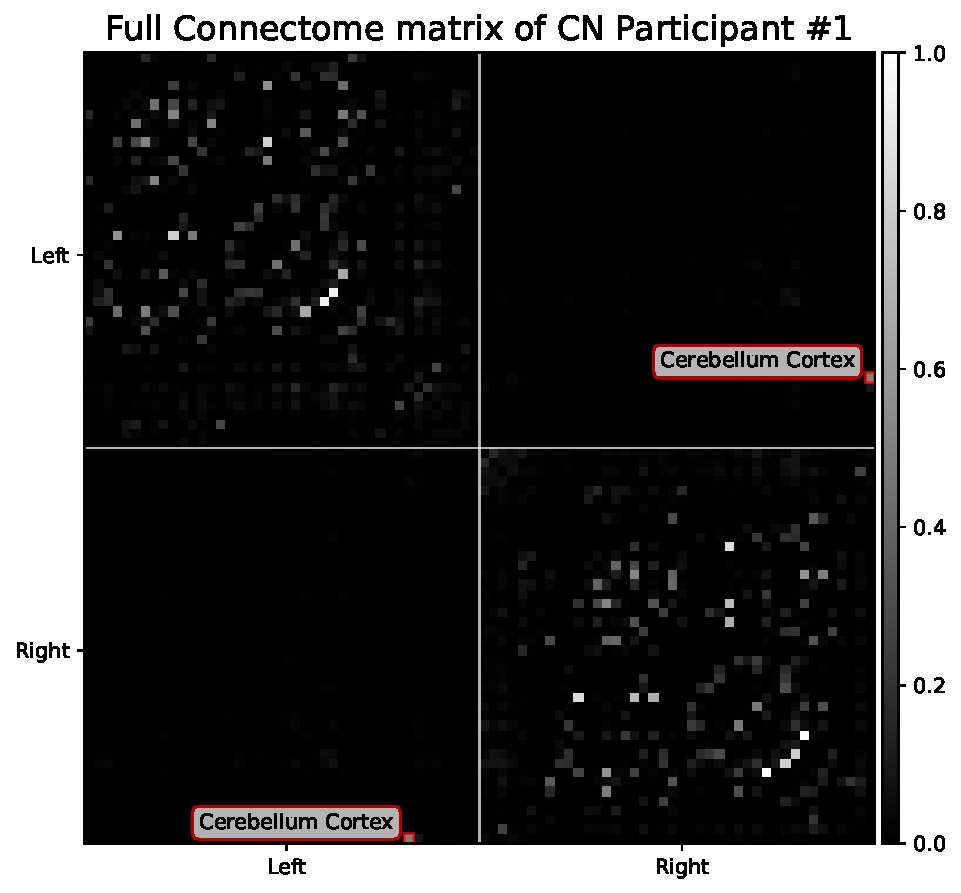
\includegraphics[width=0.8\linewidth]{figures/connectome_cn_0_full.pdf}
    \caption{Full connectome matrix.}
    \label{fig:connectome_cn_0_full}
\end{figure}

\begin{figure}[H]
    \centering
    \begin{subfigure}[a]{\linewidth}
      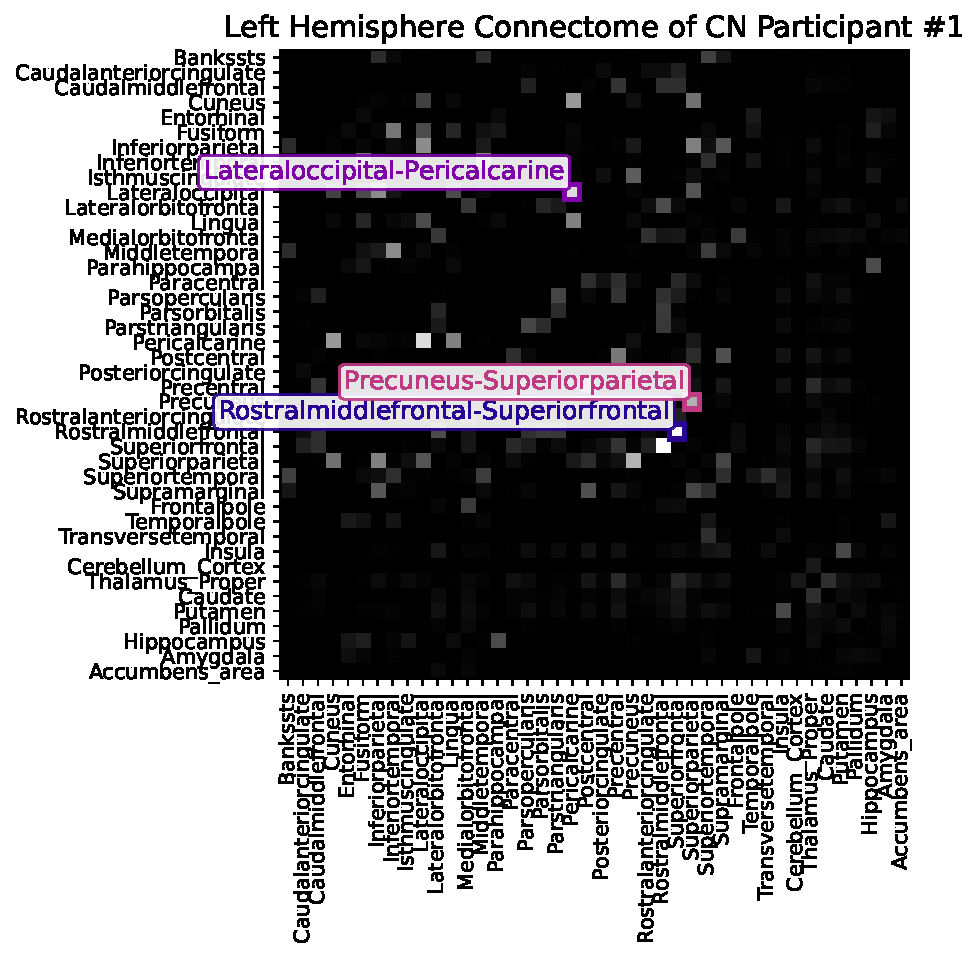
\includegraphics[width=\linewidth]{figures/connectome_cn_0_left.pdf}
      \caption{Left hemisphere.}
      \label{fig:connectome_cn_0_left}
    \end{subfigure}
    \vskip 1ex
    \begin{subfigure}[b]{\linewidth}
      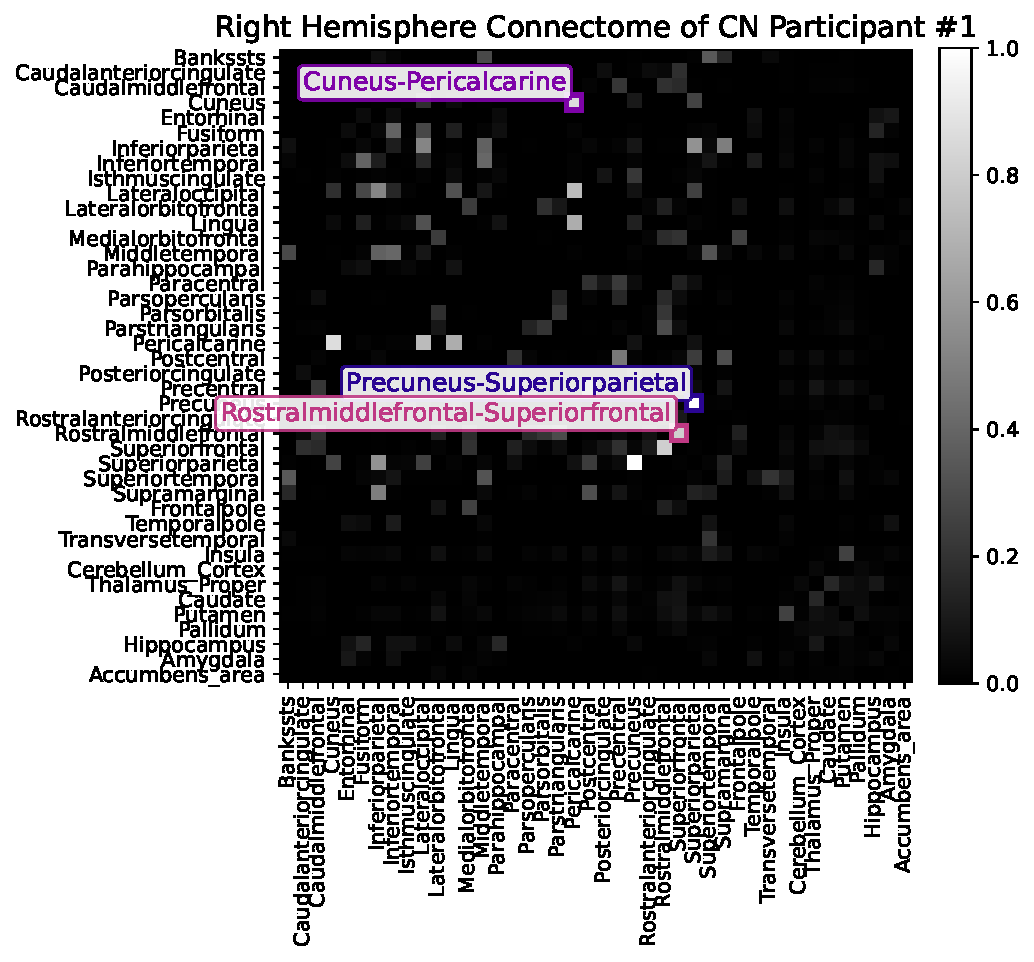
\includegraphics[width=\linewidth]{figures/connectome_cn_0_right.pdf}
      \caption{Right hemisphere.}
      \label{fig:connectome_cn_0_right}
    \end{subfigure}
    \caption{Combined connectome visualisations for a clinically normal participant.}
    \label{fig:connectome_cn_0}
\end{figure}

We then observed intra-hemispheric connectivity. Within the left hemisphere (\autoref{fig:connectome_cn_0_left}), the strongest edges link Cuneus-Pericalcarine, Precuneus-Superiorparietal and Postcentral-Precentral. We observe similar patterns in the right hemisphere (\autoref{fig:connectome_cn_0_right}), with strongest edges connecting Rostralmiddlefrontal-Superiorfrontal, Cuneus-Pericalcarine and Precuneus-Superiorparietal.

    
\begin{figure*}[b]
    \centering
    % The figure part
    \begin{tcolorbox}[colback=white, colframe=black, boxrule=0.5pt, arc=0pt]
        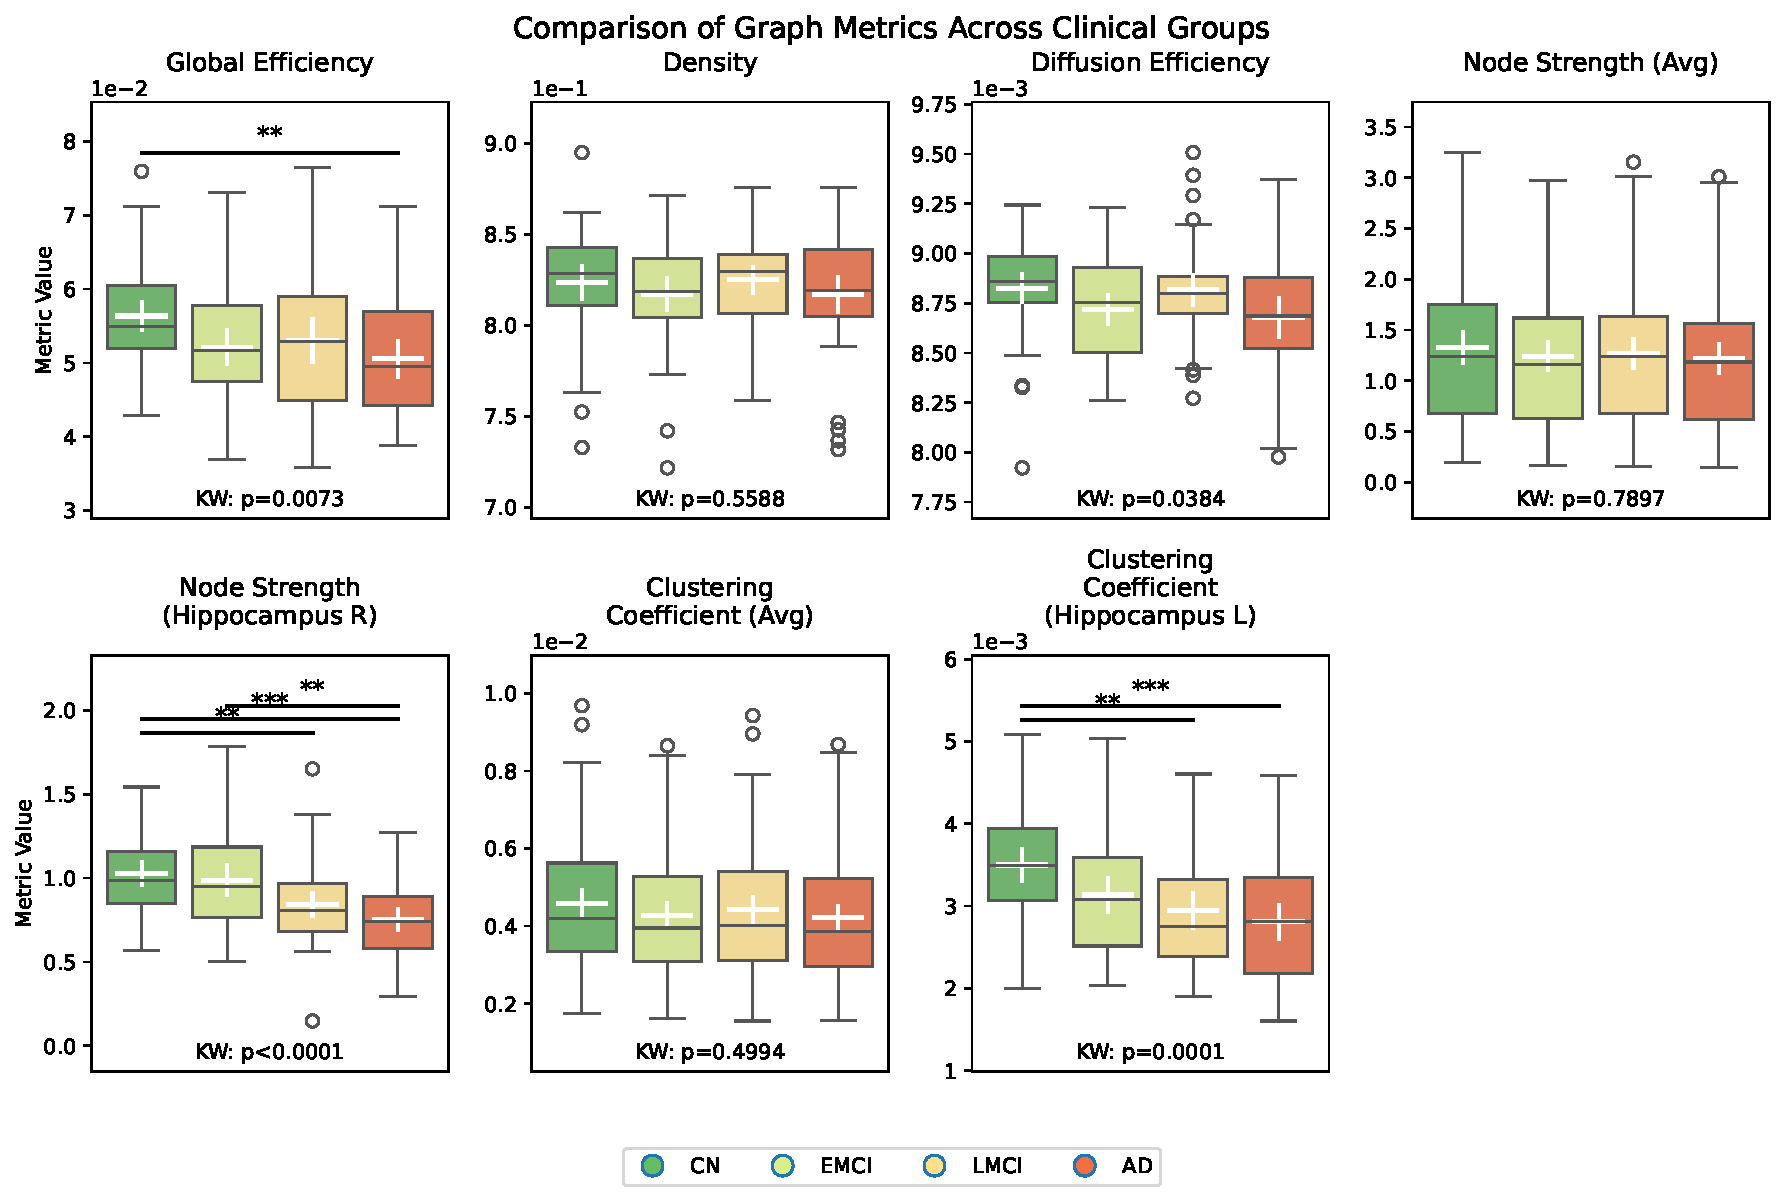
\includegraphics[width=\textwidth]{figures/graph_metrics_comparison.pdf}
        \caption{Connectome metrics for different cognitive stages. White horizontal lines indicate the group mean and vertical lines indicate the 95\% confidence intervals. Kruskal-Wallis p-values are annotated at the bottom and pairwise differences are computed using Dunn's post-hoc test. Significance indicators: * denotes p $<$ 0.05, ** denotes p $<$ 0.01, and *** denotes p $<$ 0.001.}
    
    
    \label{fig:graph_metrics_comparison}
    
    \vskip 4mm
    % The table part (without table environment)
    \small
    \captionof{table}{Significant pairwise comparisons between clinical groups}
    \label{tab:significant_comparisons}
    \begin{tabular}{lllrrrc}
        \toprule
        \textbf{Metric} & \textbf{Group 1} & \textbf{Group 2} & \textbf{Mean 1} & \textbf{Mean 2} & \textbf{\% Diff} & \textbf{p-value} \\
        \midrule
        Global Efficiency & CN & DEM & 5.64e-02 & 5.05e-02 & -10.3\% & 0.004 \\
        Node Strength (Hippocampus R) & CN & LMCI & 1.03e+00 & 8.43e-01 & -17.9\% & 0.005 \\
        Node Strength (Hippocampus R) & CN & DEM & 1.03e+00 & 7.52e-01 & -26.8\% & $<$0.001 \\
        Node Strength (Hippocampus R) & EMCI & DEM & 9.88e-01 & 7.52e-01 & -23.9\% & 0.001 \\
        Clustering Coefficient (Hippocampus L) & CN & LMCI & 3.50e-03 & 2.94e-03 & -15.9\% & 0.002 \\
        Clustering Coefficient (Hippocampus L) & CN & DEM & 3.50e-03 & 2.81e-03 & -19.7\% & $<$0.001 \\
        \bottomrule
    \end{tabular}
\end{tcolorbox}
\end{figure*}

\subsection{Connectome properties vary across different cognitive stages}\label{section:connectome_metrics_results}
We compared the connectome metrics as mentioned in \autoref{section:connectome_metrics}. 
We comment below on the metrics that show significant differences in the Dunn posthoc tests.
\begin{itemize}
    \item \textbf{Global Efficiency}: Shows significant decline (p=0.0073) as cognitive impairment progresses, with particularly strong differences between CN and AD groups (**). This suggests diminishing network integration capacity with disease progression. 
    \item \textbf{Node Strength (Right-Hippocampus)}: Displays the strongest statistical significance (p$<$0.0001) with clear stepwise decline from CN to AD, marked by multiple significant pairwise comparisons (**). This aligns with known hippocampal vulnerability in Alzheimer's disease.
    \item \textbf{Clustering Coefficient (Left-Hippocampus)}: Shows significant differences (p=0.0001) with a pronounced decrease in the AD group, indicating reduced local connectivity in this key memory-related region.
\end{itemize}




% \begin{figure*}[b]
%     \centering
%     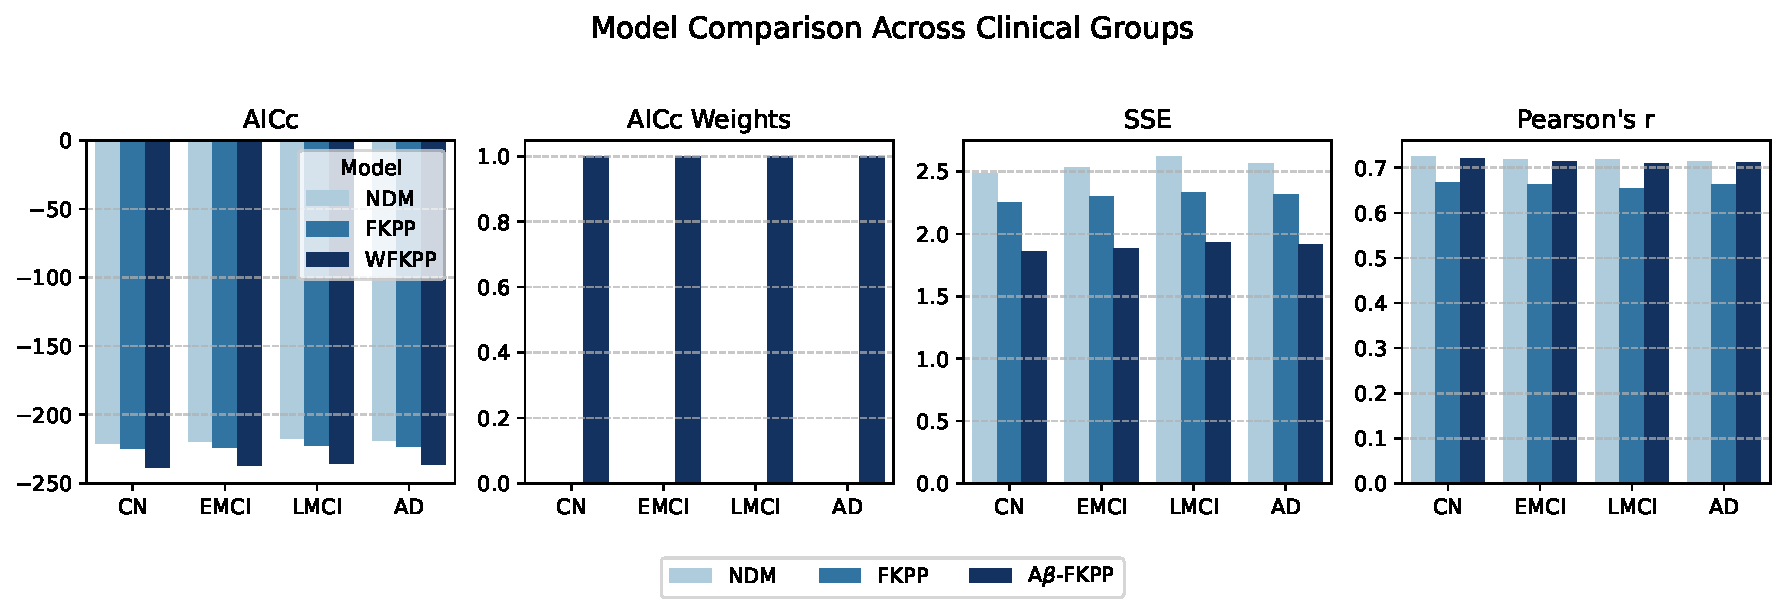
\includegraphics[width=1\linewidth]{figures/model_comparison.pdf}
%     \caption{Comparison of model performance across different cognitive stages.}
%     \label{fig:model_comparison}
% \end{figure*}

% In your preamble, ensure you have:
% \usepackage{caption}  % or \usepackage{capt-of}

\begin{figure*}[tbp]
    \begin{tcolorbox}
        \centering
        % --- Top row: main comparison figure ---
        \begin{subfigure}{\linewidth}
            \centering
            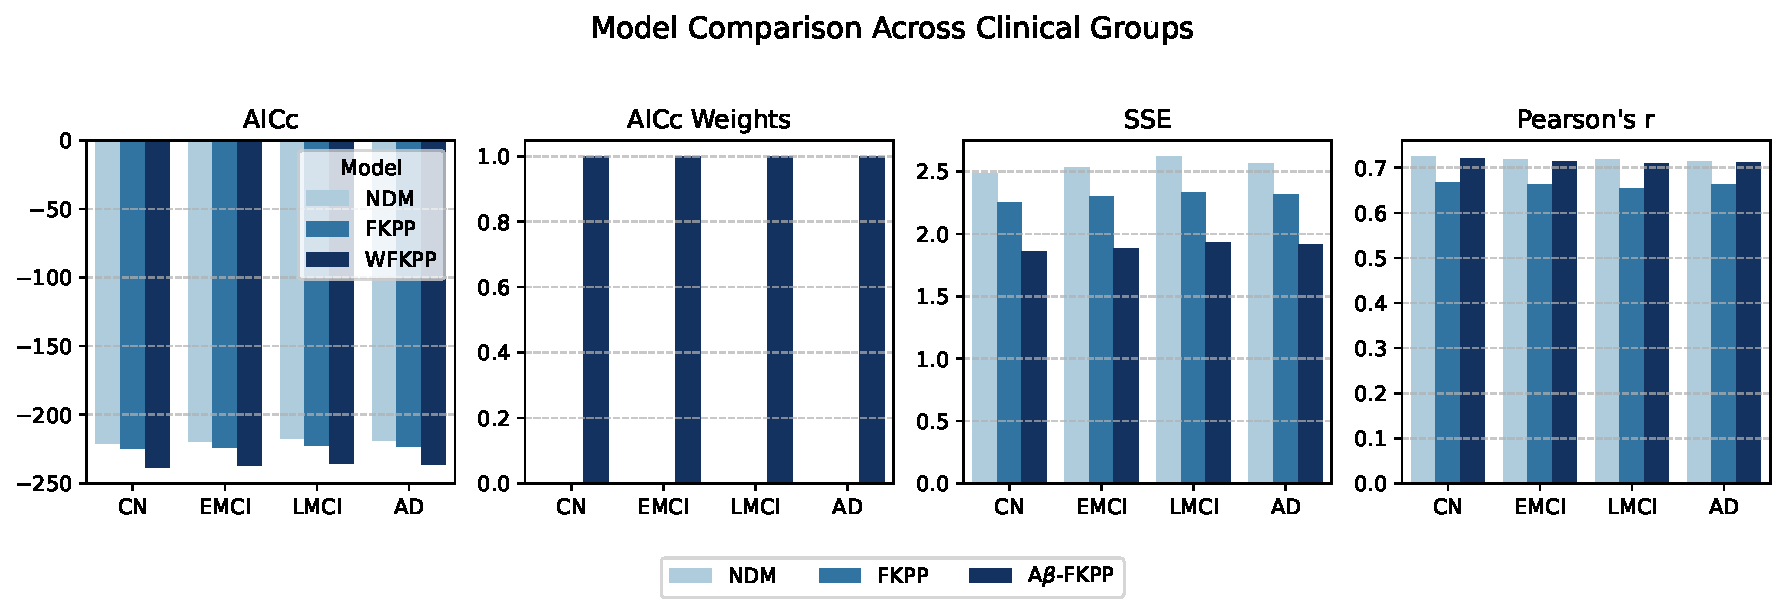
\includegraphics[width=\linewidth]{figures/model_comparison.pdf}
            \caption{Comparison of model performance across different models and cognitive stages.}
            \label{fig:model_comparison_main}
        \end{subfigure}
        
        \vspace{2em} % space before second row
        
        % --- Second row: residual plots ---
        \begin{subfigure}{0.32\linewidth}
            \centering
            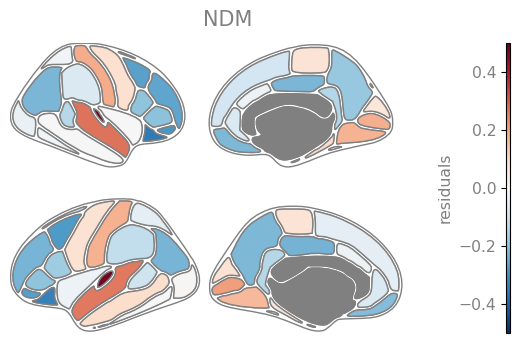
\includegraphics[width=\linewidth]{residuals_ndm_cn.png}
            \caption{NDM residuals}
            \label{fig:ndm_residuals}
        \end{subfigure}
        \hfill
        \begin{subfigure}{0.32\linewidth}
            \centering
            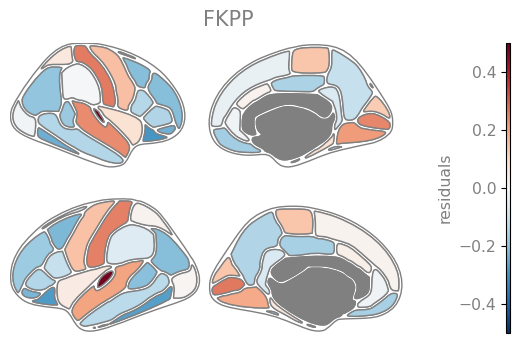
\includegraphics[width=\linewidth]{residuals_fkpp_cn.png}
            \caption{FKPP residuals}
            \label{fig:fkpp_residuals}
        \end{subfigure}
        \hfill
        \begin{subfigure}{0.32\linewidth}
            \centering
            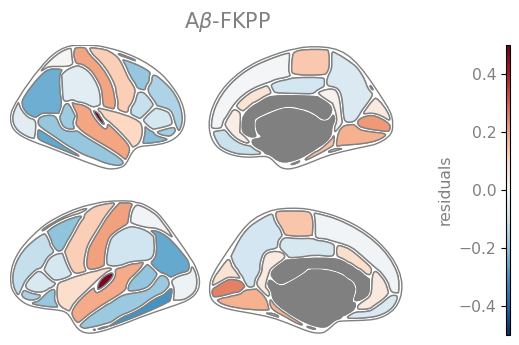
\includegraphics[width=\linewidth]{residuals_wfkpp_cn.png}
            \caption{A$\beta$-FKPP residuals}
            \label{fig:wfkpp_residuals}
        \end{subfigure}
        
        \vspace{1.5em} % Space before third row
        
        % --- Third row: correlation plots ---
        \begin{subfigure}{\linewidth}
            \centering
            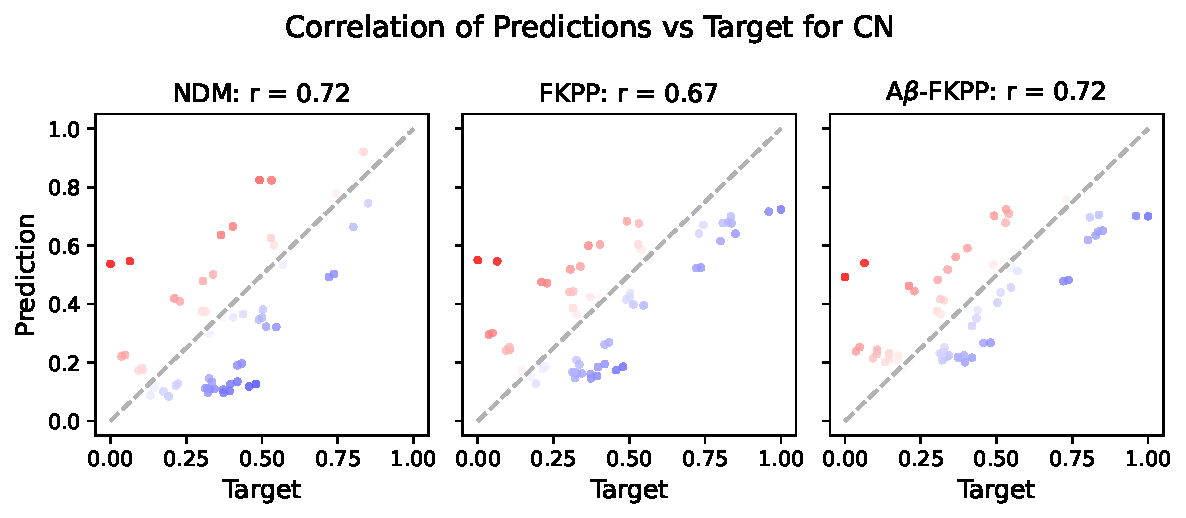
\includegraphics[width=\linewidth]{figures/correlation_prediction_vs_target_cn.pdf}
            \caption{Prediction vs target for NDM, FKPP, and A$\beta$-FKPP models in CN.}
            \label{fig:correlation_plots}
        \end{subfigure}
        
        \vspace{1.5em} % Space before fourth row
        
        % --- Fourth row: table ---
        \begin{subfigure}{\linewidth}
            \centering
            \begin{tabular}{c|p{4.5cm}|p{4.5cm}|p{4.5cm}}
                \toprule
                 & \textbf{NDM} & \textbf{FKPP} & \textbf{WFKPP} \\
                \midrule
                \multirow{3}{*}{\rotatebox[origin=c]{90}{\textbf{Over}}} &
                \textcolor{red}{Transversetemporal R} &
                \textcolor{red}{Transversetemporal R} &
                \textcolor{red}{Transversetemporal R} \\
                & \textcolor{red}{Transversetemporal L} &
                \textcolor{red}{Transversetemporal L} &
                \textcolor{red}{Transversetemporal L} \\
                & \textcolor{red}{Temporalpole R} &
                \textcolor{red}{Pericalcarine L} &
                \textcolor{red}{Pericalcarine L} \\
                \midrule
                \multirow{3}{*}{\rotatebox[origin=c]{90}{\textbf{Under}}} &
                \textcolor{blue}{Lateralorbitofrontal R} &
                \textcolor{blue}{Lateralorbitofrontal R} &
                \textcolor{blue}{Inferiortemporal L} \\
                & \textcolor{blue}{Lateralorbitofrontal L} &
                \textcolor{blue}{Lateralorbitofrontal L} &
                \textcolor{blue}{Inferiortemporal R} \\
                & \textcolor{blue}{Parsorbitalis R} &
                \textcolor{blue}{Inferiortemporal L} &
                \textcolor{blue}{Inferiorparietal L} \\
                \bottomrule
            \end{tabular}
            \caption{Regions with largest prediction errors across models in CN group}
            \label{fig:error_regions_table}
        \end{subfigure}
    \end{tcolorbox}
    \caption{Comprehensive comparison of model performance, residuals, and prediction errors.}
    \label{fig:model_comparison}
\end{figure*}
    
    

\subsection{NDM ranks best in r values}
In terms of Pearson's \(r\) values, the NDM model performs best, followed by A$\beta$-FKPP and FKPP. This indicates that NDM is more capable of capturing relative distribution of tau SUVR values across regions. We further probe this in \autoref{section:residuals_by_region}.\\

\subsection{A$\beta$-FKPP ranks best in SSE, AICc}
When comparing the models in terms of SSE, AICc and AIC, the A$\beta$-FKPP model outperforms the other two models. This suggests supports the hypothesis of A$\beta$-modulated tau accumulation.

\subsection{CN group ranks best in r, SSE}
From \autoref{tab:model_comparison_r_sse}, we observe that the CN group has the best performance in terms of both r and SSE values across all models. It could be because tau pathology is less advanced in CN individuals that the connectome network is more stable and less variable, allowing for more accurate predictions. We observe this lower variance as well in the individual connectome analysis in \autoref{tab:model_performance_distribution_individuals}. However, we acknowledge that since we do not have access to the demographics of the group-averaged tau SUVR values, there could be confounding factors unaccounted for.


\subsubsection{Predicted seeds}
Interestingly, while NDM and FKPP finds the Inferiortemporal region as the optimal seed, the A$\beta$-FKPP model finds the Entorhinal region as the optimal seed, consistent with observation that the transentorhinal cortex is the first affected area of pregressive degeneration in the medial temporal lobe, associated in early stage AD \citep{dominguez2018three}. We note here the lower $\alpha$ values, which could be attributable to the scalar impact of A$\beta$ weights and actual difference in proportions of spread contribution.



\begin{table}[h]
    \centering
    \small
    \setlength{\tabcolsep}{4pt}
    \begin{tabular}{llllll}
    \toprule
    \textbf{Group} & \textbf{Model} & \textbf{Seed} & \(\alpha\) & \textbf{SSE} & \textbf{\(r\)} \\
    \midrule
    \rowcolor{gray!15}
    CN   & NDM          & Inf. temporal & --     & 2.48 & 0.72 \\
    \rowcolor{gray!15}
    CN   & FKPP         & Inf. temporal & 0.46  & 2.25 & 0.67 \\
    \rowcolor{gray!15}
    CN   & A$\beta$-FKPP & Entorhinal   & 0.42  & 1.86 & 0.72 \\
    \midrule
    EMCI & NDM          & Inf. temporal & --     & 2.53 & 0.72 \\
    EMCI & FKPP         & Inf. temporal & 0.45  & 2.30 & 0.66 \\
    EMCI & A$\beta$-FKPP & Entorhinal   & 0.43  & 1.88 & 0.71 \\
    \midrule
    \rowcolor{gray!15}
    LMCI & NDM          & Inf. temporal & --     & 2.62 & 0.72 \\
    \rowcolor{gray!15}
    LMCI & FKPP         & Inf. temporal & 0.47  & 2.33 & 0.65 \\
    \rowcolor{gray!15}
    LMCI & A$\beta$-FKPP & Entorhinal   & 0.42  & 1.93 & 0.71 \\
    \midrule
    AD   & NDM          & Inf. temporal & --     & 2.56 & 0.72 \\
    AD   & FKPP         & Inf. temporal & 0.45  & 2.32 & 0.66 \\
    AD   & A$\beta$-FKPP & Entorhinal   & 0.41  & 1.91 & 0.71 \\
    \bottomrule
    \end{tabular}
    \caption{Comparison of models across clinical groups}
    \label{tab:model_comparison_r_sse}
\end{table}


\subsubsection{Residuals by Region}\label{section:residuals_by_region}
From \autoref{fig:correlation_plots}, the NDM model indeed exhibits a stronger linear relationship between prediction and target values.\\ 

We highlight the 3 regions with the largest overpredictions and underpredictions in \autoref{fig:error_regions_table}. All 3 models similarly have largest overpredictions for the Transeversetemporal regions on both sides. We found a distinction between the NDM and FKPP models versus the A$\beta$-FKPP model on the underpredictions. The NDM and FKPP models had the largest underprediction for the Lateralorbitofrontal regions on both sides, while the A$\beta$-FKPP model had the largest underprediction for Inferiortemporal regions on both sides, which, interestingly, corresponds to the optimal seed region for both NDM and FKPP models.\\



% \begin{figure}[H]
%     \centering
%     \begin{subfigure}[b]{0.45\linewidth}
%         \centering
%         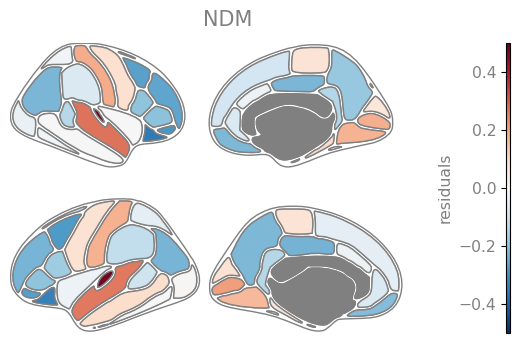
\includegraphics[width=\linewidth]{residuals_ndm_cn.png}
%         \vspace{1mm}
%         \textbf{(a)}
%     \end{subfigure}
%     \hfill
%     \begin{subfigure}[b]{0.45\linewidth}
%         \centering
%         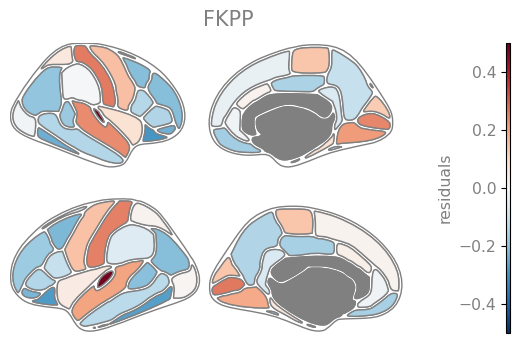
\includegraphics[width=\linewidth]{residuals_fkpp_cn.png}
%         \vspace{1mm}
%         \textbf{(b)}
%     \end{subfigure}
%     \vskip 4mm
%     \begin{subfigure}[b]{0.45\linewidth}
%         \centering
%         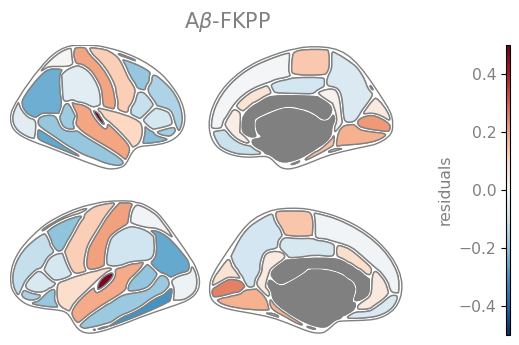
\includegraphics[width=\linewidth]{residuals_wfkpp_cn.png}
%         \vspace{1mm}
%         \textbf{(c)}
%     \end{subfigure}
%     \hfill
%     \begin{subfigure}[b]{0.45\linewidth}
%         \centering
%         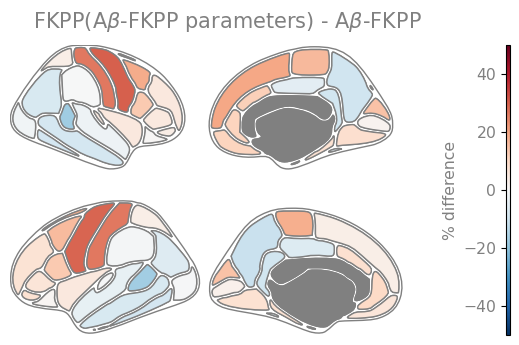
\includegraphics[width=\linewidth]{residuals_fkpp_wfkpp_diff_cn.png}
%         \vspace{1mm}
%         \textbf{(d)}
%     \end{subfigure}
%     \caption{Residuals from NDM, FKPP, A$\beta$-FKPP (panels a--c) and the difference between weighted-FKPP and FKPP (panel d).}
%     \label{fig:comparison_subfigures}
% \end{figure}

\subsubsection{Robustness testing through individual connectome analysis}
Though the NDM fit to group average connectome had better r values, we observed that the mean performance across individuals had the largest (negative) difference compared to other models, and had the largest 95 percentile ranges. The NDM also had the largest 95 percentile range of SSE values across individuals, indicating that the model fit was not robust across individuals.\\ 

A$\beta$-FKPP model had generally worse performance mean across individuals, but this may be attributable to using group-averaged A$\beta$-FKPP values that aligned better with group-averaged connectomes, and it would be interesting to see if the model fit improves when using individual A$\beta$-FKPP values.


\begin{table*}[h]
    \centering
    \small % Reduce font size slightly
    \setlength{\tabcolsep}{4pt} % Reduce column spacing
    \caption{Model performance distribution across individual connectomes}
    \label{tab:model_performance_distribution_individuals}
    \begin{tabular}{lccccccccc}
    \toprule
    & & \multicolumn{4}{c}{\textbf{SSE}} & \multicolumn{4}{c}{\textbf{Pearson's r}} \\
    \cmidrule(lr){3-6} \cmidrule(lr){7-10}
    \textbf{Group} & \textbf{Model} & \textbf{Avg} & \makecell{\textbf{Indiv.} \\ \textbf{$\mu$}} & \makecell{\textbf{\%} \\ \textbf{diff}} & \makecell{\textbf{95p Range}} & \textbf{Avg} & \makecell{\textbf{Indiv.} \\ \textbf{$\mu$}} & \makecell{\textbf{\%} \\ \textbf{diff}} & \makecell{\textbf{95p Range}} \\
    \midrule
    \rowcolor{gray!15}
    CN & NDM & 2.48 & 2.50 & 0.64 & 0.555 & 0.724 & 0.677 & \textbf{-6.97} & 0.168 \\
    \rowcolor{gray!15}
    CN & FKPP & 2.25 & 2.26 & 0.45 & 0.352 & 0.667 & 0.655 & -1.69 & 0.091 \\
    \rowcolor{gray!15}
    CN & A$\beta$-FKPP & 1.86 & 1.90 & \textbf{2.14} & 0.394 & 0.720 & 0.718 & -0.36 & 0.151 \\
    \midrule
    EMCI & NDM & 2.53 & 2.56 & 1.04 & \textbf{0.630} & 0.719 & 0.686 & -4.80 & \textbf{0.174} \\
    EMCI & FKPP & 2.30 & 2.29 & -0.36 & 0.348 & 0.663 & 0.654 & -1.36 & 0.091 \\
    EMCI & A$\beta$-FKPP & 1.88 & 1.92 & 1.90 & 0.453 & 0.713 & 0.715 & 0.20 & 0.113 \\
    \midrule
    \rowcolor{gray!15}
    LMCI & NDM & 2.62 & 2.60 & -0.53 & 0.604 & 0.718 & 0.654 & \textbf{-9.76} & \textbf{0.174} \\
    \rowcolor{gray!15}
    LMCI & FKPP & 2.33 & 2.35 & 0.83 & 0.468 & 0.654 & 0.641 & -2.03 & 0.110 \\
    \rowcolor{gray!15}
    LMCI & A$\beta$-FKPP & 1.93 & 1.96 & 1.44 & \textbf{0.662} & 0.709 & 0.706 & -0.43 & 0.141 \\
    \midrule
    AD & NDM & 2.56 & 2.61 & \textbf{1.87} & \textbf{0.809} & 0.714 & 0.656 & \textbf{-8.97} & \textbf{0.231} \\
    AD & FKPP & 2.32 & 2.32 & 0.16 & 0.505 & 0.662 & 0.645 & -2.69 & 0.126 \\
    AD & A$\beta$-FKPP & 1.91 & 1.95 & \textbf{2.09} & 0.426 & 0.712 & 0.708 & -0.58 & 0.116 \\
    \bottomrule
    \end{tabular}
\end{table*}

\subsection{Using optimal hyperparameters from the A$\beta$-FKPP model on FKPP}
The FKPP model, when forced to use the A$\beta$-FKPP model’s optimal parameters, sees an increase in SSE from 1.86 to 2.40, and a decrease in r score from 0.72 to 0.62.
We see an increase in predicted tau deposition in the Precentral and Postcentral regions, but a decrease in Bankssts and the Inferiortemporal regions. This divergence from pure FKPP suggests that the A$\beta$-modulated seed choice and growth rate emphasize certain pathways in a way that does not neatly translate into the unweighted FKPP environment. These findings underscore that parameters valid in a model incorporating amyloid load may not fully transfer to a simpler model, highlighting the importance of explicitly accounting for amyloid–tau interactions to better capture disease progression patterns.

\begin{figure}[h]
    \centering
    % First subfigure: The image
    \begin{subfigure}[b]{\linewidth}
        \centering
        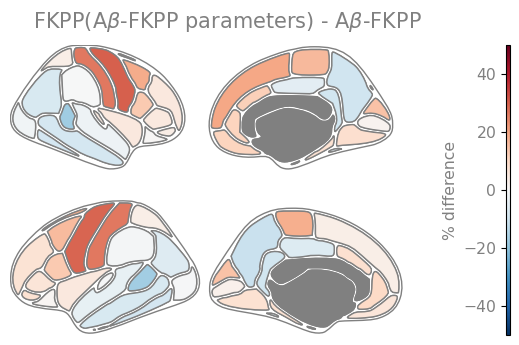
\includegraphics[width=\linewidth]{residuals_fkpp_wfkpp_diff_cn.png}
        \caption{Prediction difference between FKPP with A$\beta$ parameters versus A$\beta$-FKPP.}
        \label{fig:fkpp_wfkpp_diff}
    \end{subfigure}
    
    \vspace{1em} % Optional vertical space to separate the subfigures
    
    % Second subfigure: The table with mandatory width argument added
    \begin{subfigure}[b]{\linewidth}
        \centering
        \begin{tabular}{c|p{2.7cm}|p{1.5cm}}
            \toprule
                & \textbf{Regions} & \textbf{\% Diff} \\
            \midrule
            \multirow{3}{*}{%
                \parbox{2.3cm}{\centering \textbf{FKPP}\\ \textbf{higher}}
            }
                & \textcolor{red}{Precentral L} & 29.7\\
                & \textcolor{red}{Postcentral L} & 29.2\\
                & \textcolor{red}{Precentral R} & 26.4\\ 
            \midrule
            \multirow{3}{*}{%
                \parbox{2.3cm}{\centering \textbf{A$\beta$-FKPP}\\ \textbf{higher}}
            }
                & \textcolor{blue}{Bankssts L} &17.6\\
                & \textcolor{blue}{Bankssts R} &17.2\\
                & \textcolor{blue}{Inferiortemporal R} &11.2\\
            \bottomrule
        \end{tabular}
        \caption{Top 3 regions with largest differences between models}
        \label{tab:fkpp_wfkpp_diff}
    \end{subfigure}
    
\end{figure}

    
    

\subsection{Influence of A$\beta$ on tau production}
The null model performs significantly worse (permutation-based p-value $<$ 0.01), thus concluding that ground truth A$\beta$ is the key factor for A$\beta$-FKPP's performance. What's most interesting is the inclination towards Inferiortemporal regions as the optimal seed, which corresponds also to the optimal seeds in NDM and FKPP models, meanwhile the original Entorhinal seed was never selected.
\begin{figure}[h]
    \centering
    \begin{subfigure}[t]{0.4\linewidth}
        \centering
        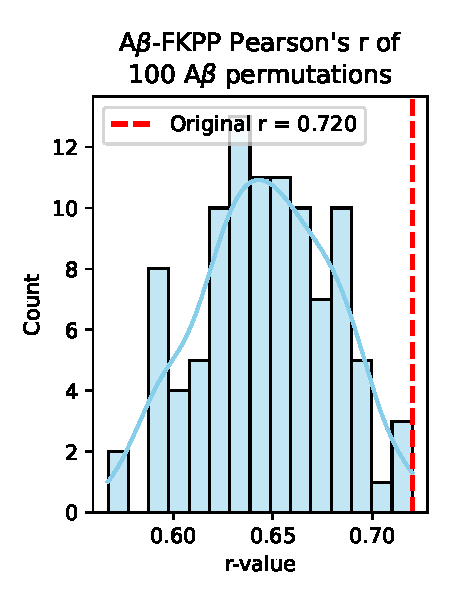
\includegraphics[width=\linewidth]{wfkpp_permuted_ab_r_distribution.pdf}
        \vspace{1mm}
        \textbf{(a)}
    \end{subfigure}
    \begin{subfigure}[t]{0.55\linewidth}
        \centering
        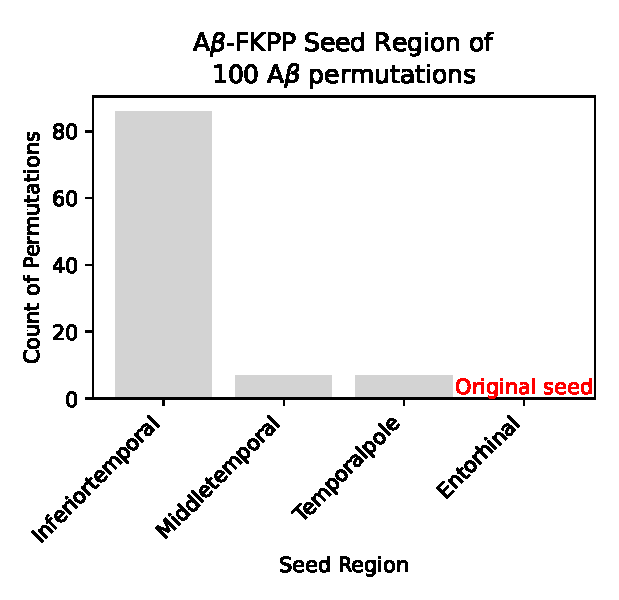
\includegraphics[width=\linewidth]{wfkpp_permuted_ab_seed_region.pdf}
        \vspace{1mm}
        \textbf{(b)}
    \end{subfigure}
    \caption{Distribution of r values when permuting the A$\beta$ weights (a) and The distribution of optimal seed regions across 100 permutations (b).}
    \label{fig:null_model_permute_ab}
\end{figure}

\subsection{The effect of the best performing cognitive group on FKPP and NDM}
In both FKPP and NDM, the null models perform significantly worse, with the best connectome a large margin away from the original, thus verifying that the original connectome is a key factor for the best performing group average connectome's performance. We also see a more diverse set of optimal seed regions chosen.
\begin{figure}[h]
    \centering
    \begin{subfigure}[t]{0.4\linewidth}
        \centering
        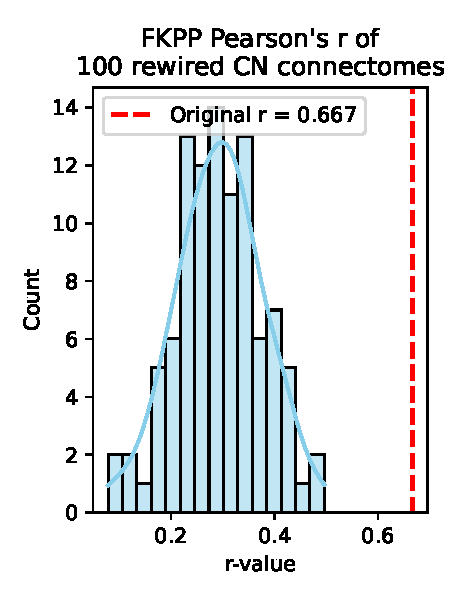
\includegraphics[width=\linewidth]{fkpp_rewired_r_distribution.pdf}
        \vspace{1mm}
        \textbf{(a)}
    \end{subfigure}
    \begin{subfigure}[t]{0.55\linewidth}
        \centering
        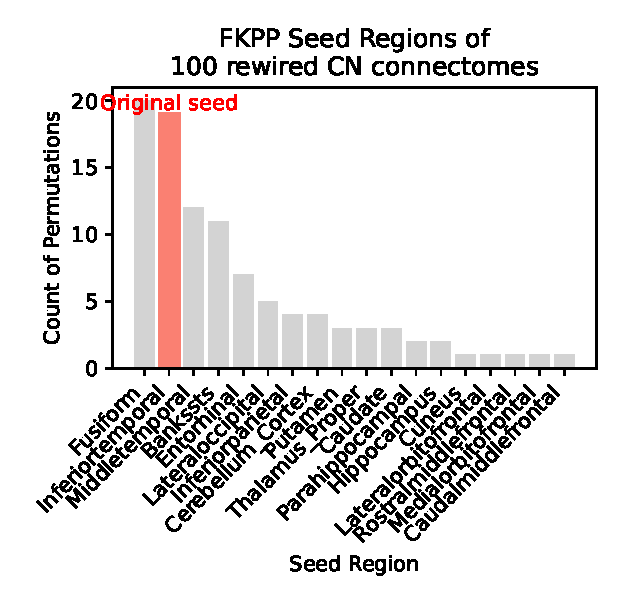
\includegraphics[width=\linewidth]{fkpp_rewired_seed_region.pdf}
        \vspace{1mm}
        \textbf{(b)}
    \end{subfigure}
    \vskip 4mm
    \begin{subfigure}[t]{0.4\linewidth}
        \centering
        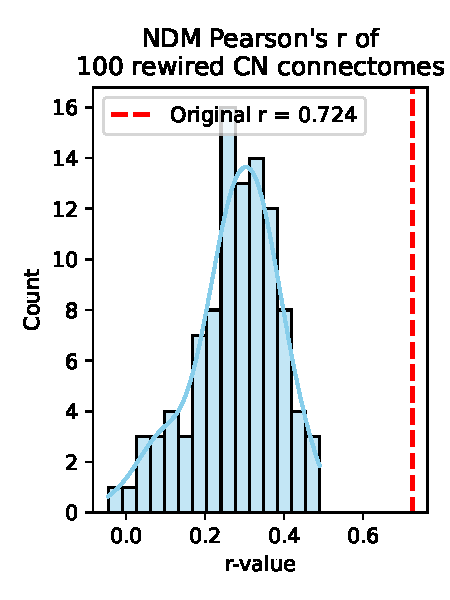
\includegraphics[width=\linewidth]{ndm_rewired_r_distribution.pdf}
        \vspace{1mm}
        \textbf{(c)}
    \end{subfigure}
    \begin{subfigure}[t]{0.55\linewidth}
        \centering
        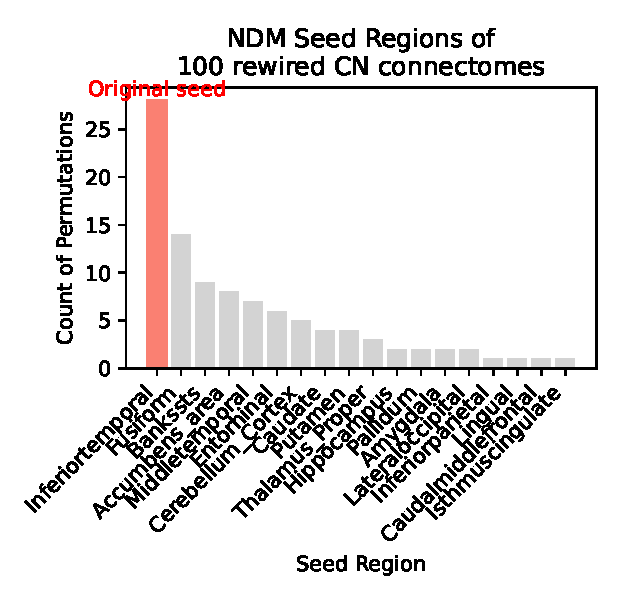
\includegraphics[width=\linewidth]{ndm_rewired_seed_region.pdf}
        \vspace{1mm}
        \textbf{(d)}
    \end{subfigure}
    \caption{Distribution of r values when rewiring connectomes (a) and The distribution of optimal seed regions across 100 permutations (b).}
    \label{fig:null_model_rewire_connectomes}
\end{figure}





\section{Discussion}
\label{sec:Discussion}

\subsection{Network Model Performance}
Our comparative results demonstrate that tau propagation in AD can be reasonably well predicted by connectome-based models across the clinical continuum. In particular, the simple Network Diffusion Model (NDM) performed almost as well as a more complex reaction–diffusion model in explaining a canonical tau distribution, highlighting that the brain’s network architecture is a primary determinant of where tau pathology accumulates. In fact, the simplest model NDM captures the relative tau-levels across regions best, with highest r-scores. This finding resonates with the view that brain networks serve as conduits for disease spread, constraining tau to follow connectivity routes. 

\subsection{Amyloid-$\beta$ Influences tau Accumulation}
The significant improvement in performance when incorporating A$\beta$ into the weighted FKPP supports the hypothesis that Amyloid-$\beta$ Influences tau Accumulation. A notable distinction also emerged in the optimal seed regions identified. While both NDM and FKPP converged on the Inferiortemporal region as the optimal seed, the A$\beta$-FKPP model consistently identified the Entorhinal region instead. This finding aligns remarkably well with established neuropathological staging, where the transentorhinal cortex represents the initial site of tau pathology in early Alzheimer's disease progression \citep{dominguez2018three}.

\subsection{Clinically Normal Most Robust Predictions}
Another important result from our study is that model performance varied across individual connectomes, even within the same diagnostic group. While we used group-averaged metrics to compare models, the spread in Pearson r values for individuals (see Table 3) reveals that some participants’ brain networks predicted the tau pattern considerably better than others. The CN group both has better model performance across models and lowest variance in distribution of individual connectome performance. 

\subsection{Limitations}
A key limitation of our study is the use of a group-averaged tau PET map (from 242 individuals) as the ground truth for model fitting, irrespective of cognitive stage. While this provided a uniform comparison metric, it introduced a potential confound. The “tau-positive” PET cohort likely had a distribution of ages and disease stages that do not perfectly align with the CN, MCI, and AD sub-groups whose connectomes we used. Differences in age, amyloid status, vascular health, and other factors between the connectome donors and the tau-PET cohort could influence results. For example, we found that CN connectomes have higher global efficiency and node strength in the hippocampus than AD connectomes. We control for this by evaluatin against null models, but acknowledge that this does not account for all possible confounds.



\bibliographystyle{acl_natbib}
\bibliography{acl2021}


\end{document}
